\documentclass[a4paper, 11pt, margin=1in]{journal}
\usepackage[a4paper, total={6in, 8in}]{geometry}
\usepackage[utf8]{inputenc}
\usepackage{multicol}
\usepackage{fancyvrb}
\usepackage{graphicx}
% redefine \VerbatimInput
\RecustomVerbatimCommand{\VerbatimInput}{VerbatimInput}%
{fontsize=\footnotesize,
 %
 frame=lines,  % top and bottom rule only
 framesep=2em, % separation between frame and text
 %
 label=\fbox{Model summary},
 labelposition=topline,
 %
 commandchars=\|\(\), % escape character and argument delimiters for
                      % commands within the verbatim
 commentchar=*        % comment character
}
\setlength{\textheight}{674pt}


\newcommand{\authorx}{Palomo Alonso, Alberto}
\newcommand{\noreport}{CNET0047}
\newcommand{\name}{model 0}
\newcommand{\dbname}{wikipedia dataset}
\newcommand{\dbtype}{BaseNetDatabase (BND) }
\newcommand{\dbsize}{132864}
\newcommand{\dbdist}{(0.6999036608863198, 0.15028901734104047, 0.1498073217726397)}
\newcommand{\modeli}{(8, 8, 1)}
\newcommand{\modelo}{8}
\newcommand{\modelloss}{mean squared error}
\newcommand{\modelopt}{adam}
\newcommand{\modeldevs}{1}
\newcommand{\modeltab}{Flatten & (None,) &  \\ 
Dense & (128,) &  \\ 
Dense & (64,) &  \\ 
Dense & (32,) &  \\ 
}
\newcommand{\maxloss}{0.0276}
\newcommand{\minloss}{0.0255}


\title{\textbf{Automatic generated report \noreport.}}
\author{Author: \authorx\\ Date of submission: \today.}

\begin{document}
\pagestyle{empty}
\maketitle
\vspace{1cm}
\raggedright

\begin{figure}[h!]
    \centering
    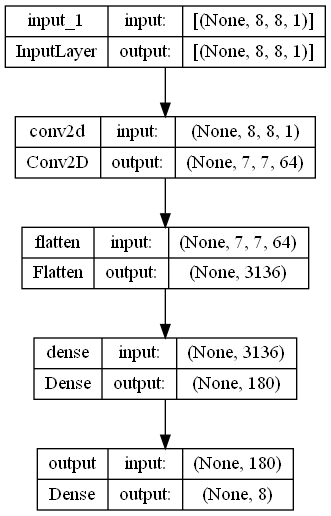
\includegraphics[height=16cm]{imgs/model}
    \caption{Model visualization}
\end{figure}

\section{Model}

The model has been compiled successfully with the following parameters:\\
\vspace{1cm}

\begin{table*}[h!]
    \centering
    \begin{tabular}{|l|l|l|}
        \hline
        \textbf{Layer}                 & \textbf{Shape}                 & \textbf{Attributes}                              \\
        \hline
         \modeltab
         \hline
    \end{tabular}
    \caption{Model architecture and attributes.}
\end{table*}

\vspace{1cm}
\VerbatimInput{summary.txt}

\newpage
\subsection{Compiler}

\begin{itemize}
    \item \textit{Problem specifications.} The input shape mesh is (\textit{\modeli}), while the output shape is (\textit{\modelo}).
    \item \textit{Compiling options.} The model makes use of the \textit{\modelloss} loss function and the \textit{\modelopt} optimizer. The metrics taken into account are accuracy and loss.
    \item \textit{Devices.} The model was trained with \modeldevs GPUs.
\end{itemize}
\section{Database}

The database \textbf{\dbname} was generated with \textit{\dbtype}. The training - validation - test distribution is \textit{\dbdist} and the total size of the database is \textit{\dbsize}. 

\section{Performance}

The obtained learning curve is shown below. With \textbf{maxloss}: \maxloss, and \textbf{minloss}: \minloss.\\
\end{document}

\begin{figure}
    \centering
    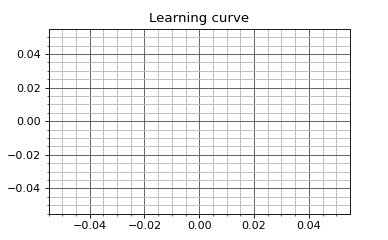
\includegraphics[height=6cm]{imgs/learning}
    \caption{Learning curve with the introduced database.}
\end{figure}